
%\documentclass[calculator,steamtables,datasheet,solutions]{exam}
\documentclass[calculator,fluidstables,allquestions,datasheet]{exam}

% The full list of class options are
% calculator : Allows approved calculator use.
% datasheet : Adds a note that data sheet are attached to the exam.
% handbook : Allows the use of the engineering handbook.
% resit : Adds the resit markings to the paper.
% sample : Adds conspicuous SAMPLE markings to the paper
% solutions : Uses the contents of \solution commands (and \solmarks) to generate a solution file

\usepackage{pdfpages} 
\usepackage{lscape,comment}
 
\coursecode{EG3029}%%

\examtime{09.00--12.00}%
\examdate{12}{12}{2014}% 
\examformat{Candidates must attempt \textit{all} questions.}

\newcommand{\frc}{\displaystyle\frac}
\newcommand{\br}[1]{\!\left( #1 \right)}
\newcommand{\abs}[1]{\left| #1 \right|}
\newcommand{\fracd}[2]{\frac{\mathrm{d} #1}{\mathrm{d} #2}}
\newcommand{\fracp}[2]{\frac{\partial #1}{\partial #2}}
\renewcommand{\d}[1]{\mathrm{d} #1 } 
\newcommand{\Ma}{\mathrm{M\!a}} 



\begin{document}

%%%
%%% Question 01
%%%
\begin{question}
%
\begin{enumerate}[(a)]
% (Shapiro 2.34) 
\item Air contained in a piston-cylinder system undergoes three consecutive processes,
\begin{itemize} 
\item Process 1--2: Isobaric cooling with P$_{1}$=69 kPa and V$_{1}$=0.11 m$^{3}$;
\item Process 2--3: Isochoric heating with P$_{3}$=345 kPa;
\item Process 3--1: Polytropic expansion, with $PV=$ {\it constant}. %Expansion to the initial state, during which the pressure-volume relationship is $PV=$ {\it constant}.
\end{itemize}  
\begin{enumerate}[(i)]
\item Calculate V$_{2}$ $\left(\text{in m}^{3}\right)$.~\marks{4} 
\solution{
For Process 2--3: V$_{2}$=V$_{3}$. However the expansion 3--1 follows $PV=$ constant,
\begin{displaymath}
P_{1}V_{1}=P_{3}V_{3} \Longrightarrow V_{3} = \frc{P_{1}V_{1}}{P_{3}} = {\bf 0.022\;\text{m}^{3} = V_{2}}
\end{displaymath}~\solmarks{4/4}
}
\item Calculate the work (in $kJ$) for each process.~\marks{6}
\solution{\noindent
Process 1--2: 
\begin{displaymath}
{\bf W_{1-2}} = \int\limits_{V_{1}}^{V_{2}} P dV = P\left(V_{2}-V_{1}\right) = -6072 J \Rightarrow {\bf -6.072 kJ}
\end{displaymath}~\solmarks{2/6}
\noindent
Process 2--3: V$_{2}$=V$_{3}$ $\Longrightarrow$ {\bf W$_{2-3}$ = 0}~\solmarks{2/6} \\
\noindent
Process 3--1: $PV = C$
\begin{displaymath} 
{\bf W_{31}} = \int\limits_{V_{3}}^{V_{1}}P dV = \int\limits_{V_{3}}^{V_{1}}\frc{C}{V} dV = P_{1}V_{1}\ln\frc{V_{1}}{V_{3}} = 12220 J \Rightarrow {\bf 12.22 kJ} 
\end{displaymath}~\solmarks{2/6}
}
\item Sketch the $PV$ diagram for these processes.~\marks{4}
\solution{\solmarks{4/4}
\begin{center}
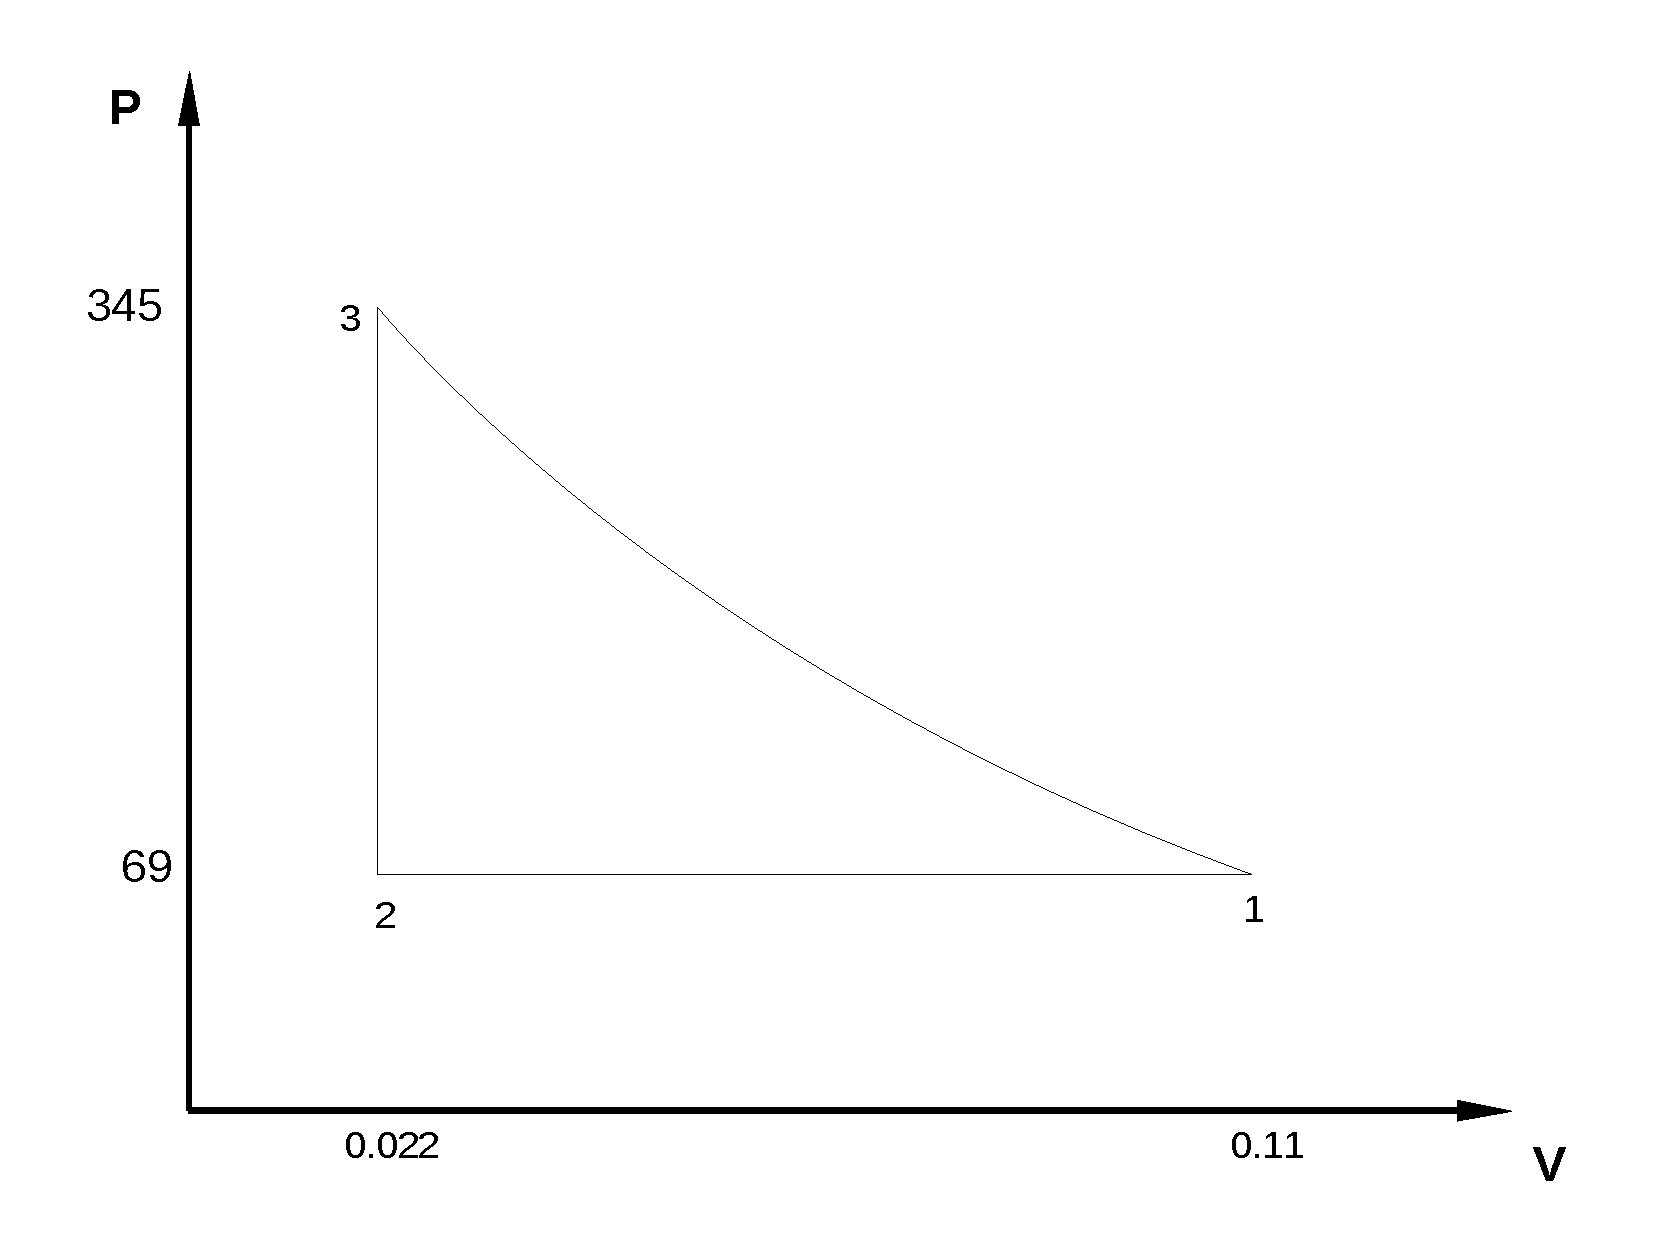
\includegraphics[width=10.cm,height=8.cm,clip]{./Pics/Exam_PV_Diagram}
\end{center}
}
\end{enumerate}
%
\item A closed system with 0.09 kg of air undergoes a polytropic process from P$_{1}$ = 138 kPa, v$_{1}$=0.72 m$^{3}$.kg$^{-1}$ to a final state where P$_{2}$ = 552 kPa, v$_{2}$ = 0.25 m$^{3}$.kg$^{-1}$.  Determine the work (in $kJ$) required for this compression.~\marks{6} 
\solution{
First stage is to calculate the polytropic coefficient,
\begin{displaymath}
P_{1}v_{1}^{n} = P_{2}v_{2}^{n} \Longrightarrow {\bf n} = \frc{\ln P_{2}/P_{1}}{\ln v_{1}/v_{2}} {\bf = 1.31}
\end{displaymath}~\solmarks{2/6}
Now, calculating the work with $V_{i}=v_{i}\times m$, thus V$_{1}=0.0648$ m$^{3}$ and V$_{2}=0.0225$ m$^{3}$:
\begin{eqnarray}
{\bf W }&=& \int\limits_{V_{1}}^{V_{2}} P dV = \int\limits_{V_{1}}^{V_{2}} \frc{C}{V^{n}} dV = \left.C \frc{V^{1-n}}{1-n}\right|_{V_{1}}^{V_{2}} = \frc{P_{2}V_{2}^{n}V_{2}^{1-n}-P_{1}V_{1}^{n}V_{1}^{1-n}}{1-n} = \frc{P_{2}V_{2}-P_{1}V_{1}}{1-n} \nonumber \\
   &=& {\bf -11.214 kJ} \nonumber
\end{eqnarray} ~\solmarks{4/6}
}
%
\end{enumerate}
%
\end{question}
\clearpage

%%%
%%% Question 02
%%%
\begin{question}
%
A geothermal power station (Rankine cycle) uses propane $\left(\text{n-C}_{3}\right)$ as working fluid to produce power $\left(W_{T}\right)$ in a turbine (isentropic expansion) with efficiency $\left(\eta_{T}\right)$ of 90$\%$. n-C$_{3}$ is vaporised by geothermal water (brine, $A-B$ in the diagram) at 90$^{\circ}$C. After condensed, n-C$_{3}$ is driven to a heat exchanger (with thermal efficiency of 68$\%$) and the cycle continues. The mass flow rate of n-C$_{3}$ $\left(\dot{m}_{C3}\right)$ is 250 kg.s$^{-1}$ and the heat capacity at constant pressure $\left(C_{p}\right)$ of brine is 3565.5 J.(kg.K)$^{-1}$. Conditions for n-C$_{3}$ and brine flows are described in Table below.
%\vspace{-.9cm}
\begin{center}
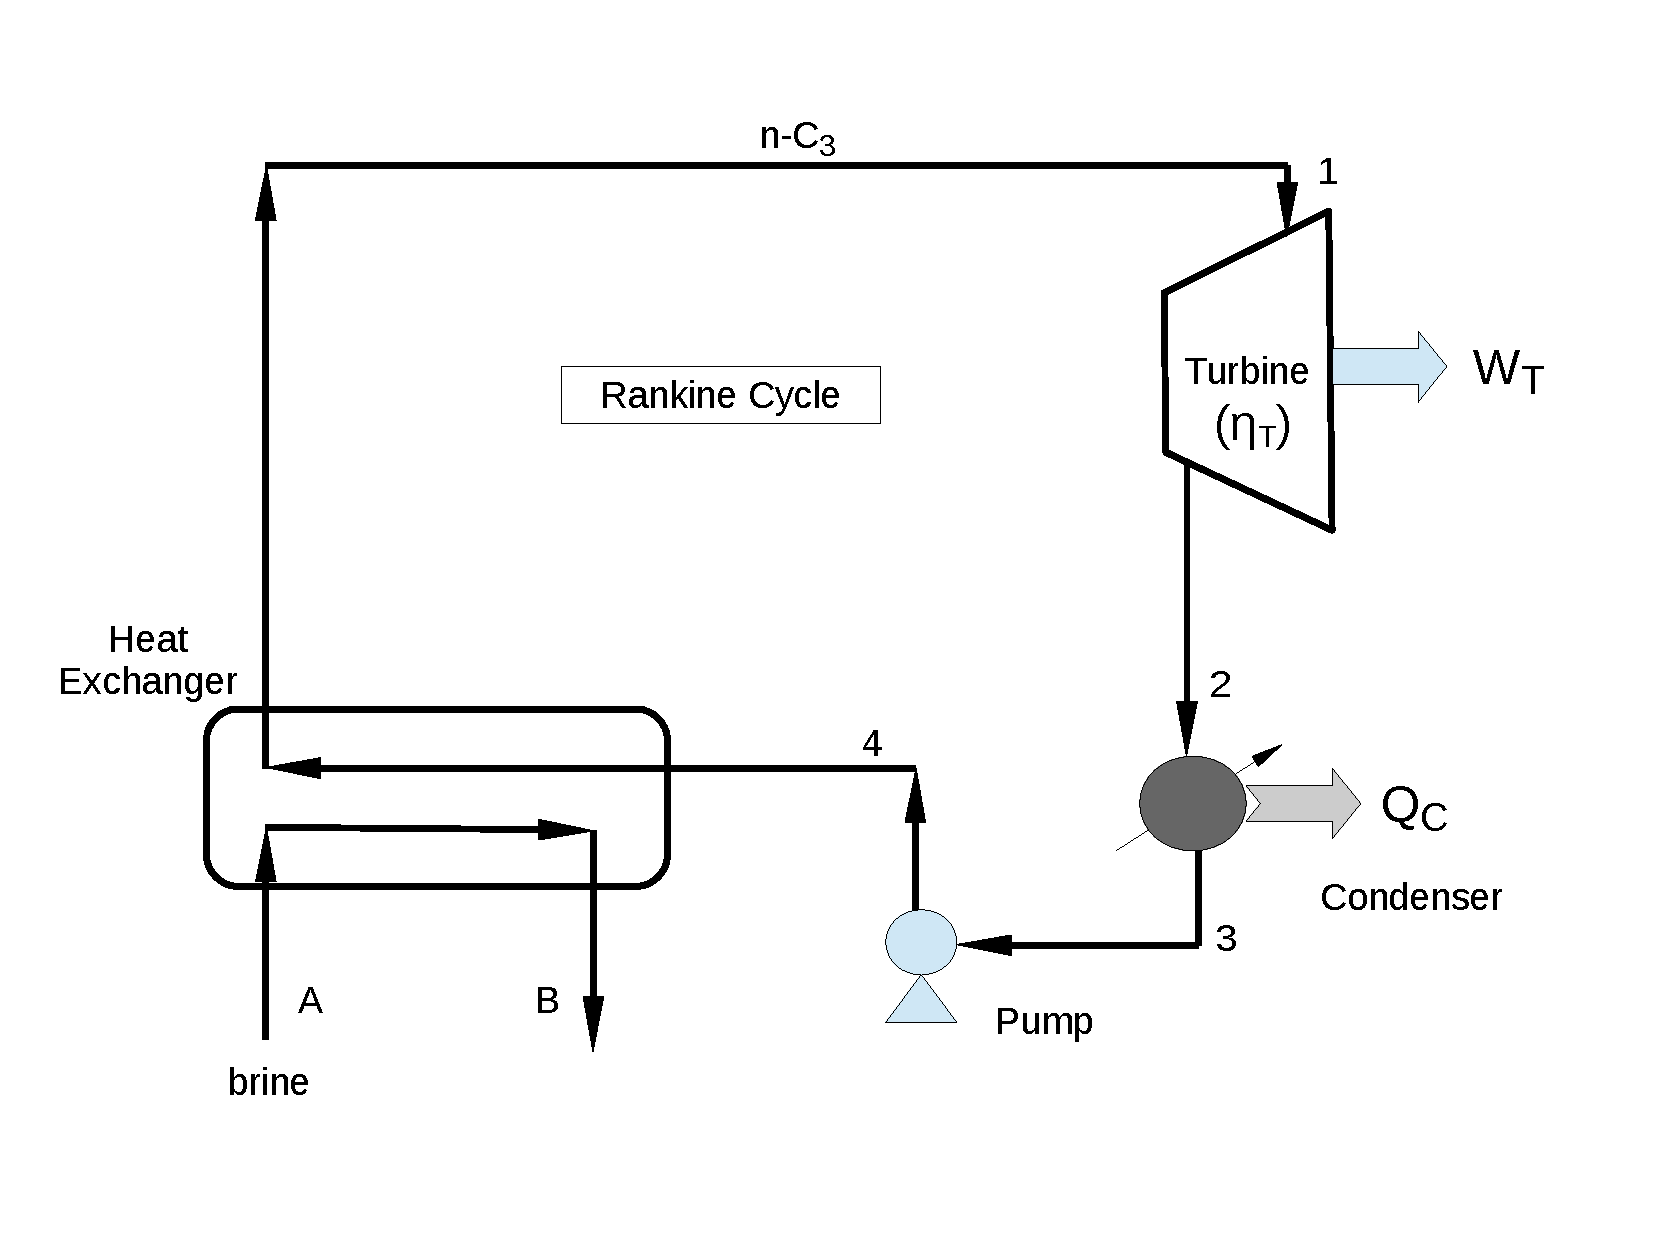
\includegraphics[width=10.cm,height=7.cm,clip]{./Pics/RankineCycle}
%\caption{ Reheat and regenerative Rankine cycle with 2 turbines.}
%\label{exam_mod02_rankinecycle}
\end{center}
%\vspace{-1.5cm}
\begin{center}
\begin{tabular} {||c | c c c c c || }
\hline\hline
{\bf Stage} & {\bf P}    & {\bf T}        & {\bf State}    & {\bf H}             & {\bf S}                  \\
            & {\bf (bar)}& {\bf ($^{o}$C)} &               & {\bf (kJ.kg$^{-1}$)} & {\bf (kJ.(kg.K)$^{-1}$)}  \\
\hline\hline
 {\bf 1 }   & 16         & 50             &   {\bf (a)}    & {\bf (b)}           & {\bf (c)}                \\
 {\bf 2 }   & 6          &  --            &   wet vapour   & {\bf (d)}           & --                       \\
 {\bf 3 }   & 6          &                &   sat. liquid  & {\bf (e)}           & --                       \\
 {\bf 4 }   & 16         &                &   {\bf (f)}    & {\bf (g)}           & --                       \\
 {\bf A }   & --         & 90             &   --           & --                  & --                       \\
 {\bf B }   & --         & 30             &   --           & --                  & --                       \\
 \hline\hline
\end{tabular}
\end{center}

\begin{enumerate}[(a)]
%%
%% Question A
%%
\item In this Table, determine {\it (a)-(g)}.~\marks{7}
%
\solution{
In order to fill the Table we need to calculate the thermodynamic properties for each stage of the cycle:
\begin{description}
%%%
\item[Stage 1:] At P$_{1}$ = 16 bar, T$_{1}$ = 50$^{\circ}$C $>$ T$_{sat}\left(P_{1}\right)$ = 46.89$^{\circ}$C. Therefore the fluid is at {\bf superheated state}~\solmarks{1/7}. From the superheated table for n-C$_{3}$ at P$_{1}$ and T$_{1}$, we can obtain:\\
{\bf H$_{1}$ = 522.5 kJ.kg$^{-1}$}~\solmarks{1/7} and\\
{\bf S$_{1}$ = 1.733 kJ.(kg.K)$^{-1}$}~\solmarks{1/7}. 
%%%
\item[Stage 2:] At P$_{2}$ = 6 bar, the fluid is wet vapour after the isentropic expansion. We should first calculate the quality of the vapour in an ideal expansion (using values of entropy/enthapy obtained from the saturated n-C$_{3}$ table at P$_{2}$.
\begin{displaymath}
x_{2s} =\frc{S_{2s}-S_{f}}{S_{g}-S_{f}} = \frc{1.733 - 0.446}{1.737-0.446} = 0.9969
\end{displaymath}
now to calculate the ideal enthalpy,
\begin{displaymath}
x_{2s} = 0.9969 = \frc{H_{2s}-H_{f}}{H_{g}-H_{f}} = \frc{H_{2s}-115.3}{478.3-115.3}\;\;\Longleftrightarrow\;\; H_{2s} = 477.17 \frc{kJ}{kg}
\end{displaymath}
As the efficiency of the turbine is of 90$\%$,
\begin{displaymath}
\eta_{\text{Turbine}} = 0.90 =\frc{H_{2}-H_{1}}{H_{2s}-H_{1}} = \frc{H_{2} - 522.5}{477.17 - 522.5} \;\;\Longleftrightarrow \;\; {\bf H_{2} = 481.70\frc{kJ}{kg}}
\end{displaymath}~\solmarks{1/7}
%%%
\item[Stage 3:] At P$_{3}$ = P$_{2}$ = 6 bar, the fluid leaving the condenser towards the pump is saturated liquid, and the enthalpy and specific volume are the same of the liquid phase obtained from the saturated table:\\
{\bf H$_{3}$} = H$_{f}\left(\text{P = 6 bar}\right)$ {\bf = 115.3 kJ.kg$^{-1}$}~\solmarks{1/7} \\
V$_{3}$ = V$_{f}\left(\text{P = 6 bar}\right)$ = 1.931$\times$10$^{-3}$ m$^{3}$.kg$^{-1}$ 
%%%
\item[Stage 4:] The fluid leaving the pump is {\bf sub-cooled liquid}.~\solmarks{1/7} As there is no heat loss in the pump, we can assume $dH \approx VdP$, therefore
\begin{displaymath}
{\bf H_{4}} = H_{3} + V_{3}\left(P_{4}-P_{3}\right) = 115.3\frc{kJ}{kg} + 1.931\times 10^{-3} \frc{m^{3}}{kg} \left(16 - 6\right)\text{bar} {\bf= 117.23 \frc{kJ}{kg}}
\end{displaymath}~\solmarks{1/7}

\end{description}
Thus the Table becomes:
\begin{center}
\begin{tabular} {||c | c c c c c || }
\hline\hline
{\bf Stage} & {\bf P}    & {\bf T}        & {\bf State}    & {\bf H}             & {\bf S}                  \\
            & {\bf (bar)}& {\bf ($^{o}$C)} &               & {\bf (kJ.kg$^{-1}$)} & {\bf (kJ.(kg.K)$^{-1}$)}  \\
\hline\hline
 {\bf 1 }   & 16         & 50             &{\bf superheated vapour}&{\bf 522.5}  & {\bf 1.733}              \\
 {\bf 2 }   & 6          &  --            &   wet vapour   & {\bf 481.70}        & --                       \\
 {\bf 3 }   & 6          &                &   sat. liquid  & {\bf 115.3}         & --                       \\
 {\bf 4 }   & 16         &                &{\bf sub-cooled liquid}& {\bf 117.23} & --                       \\
 {\bf A }   & --         & 90             &   --           & --                  & --                       \\
 {\bf B }   & --         & 30             &   --           & --                  & --                       \\
 \hline\hline
\end{tabular}
\end{center}
}
%%
%% Question B
%%
\item Calculate the power produced by the turbine $\left(W_{T}\right)$ and the heat extracted in the condenser $\left(Q_{C}\right)$ in {\it MW}.~\marks{4}
%
\solution{
\begin{displaymath}
{\bf W_{T}} = \dot{m}_{C3} \left(H_{1}-H_{2}\right) = 250\frc{kg}{s} \times \left(522.5 - 481.70\right)\frc{kJ}{kg} = 10200 \frc{kJ}{s} {\bf = 10.2 MW}
\end{displaymath}~\solmarks{2/4}

\begin{displaymath}
{\bf Q_{C}} = \dot{m}_{C3} \left(H_{2}-H_{3}\right) = 250\frc{kg}{s} \times \left(481.70 - 115.30\right)\frc{kJ}{kg} = 91600 \frc{kJ}{s} {\bf = 91.6 MW}
\end{displaymath}~\solmarks{2/4}
} 
%%
%% Question C
%%
\item Calculate the mass flow rate of brine in {\it kg.s}$^{-1}$.~\marks{6}
%
\solution{
The heat extracted by the n-C$_{3}$ $\left(\dot{Q}_{C3}\right)$ fluid in the heat exchanger can be easily calculated by
\begin{displaymath}
{\bf \dot{Q}_{C3}} = \dot{m}_{C3}\left(H_{1}-H_{4}\right) {\bf = 101317.5\frc{kJ}{s}}
\end{displaymath}~\solmarks{2/6}
Assuming that the heat extracted from the geothermal fluid (brine), $\dot{Q}_{gf}$ is transferred to the n-C$_{3}$ stream with efficiency of 68$\%$,
\begin{displaymath}
\eta_{\text{HE}} = 0.68 = \frc{\dot{Q}_{C3}}{\dot{Q_{gf}}} \;\; \Longleftrightarrow  {\bf \dot{Q}_{gf} = 148996.32 \frc{kJ}{s}}
\end{displaymath}~\solmarks{2/6}
With the heat generated by the geothermal fluid and the inlet/outlet fluid temperatures, we can now calculate the brine mass flow rate for the associated heat transferred,
\begin{displaymath} 
\dot{Q}_{gf} = 148996.32 \frc{kJ}{s} = \dot{m}_{gf} C_{p} \left(T_{A} - T_{B}\right)  \;\;\Longleftrightarrow\;\; {\bf \dot{m}_{gf} = 696.57\frc{kg}{s}}
\end{displaymath}~\solmarks{2/6}
}
%%%
%%% Question D
%%%
\item Sketch the temperature $\times$ entropy (TS) diagram for the process indicating the liquid and vapour saturated lines and each stage of the n-C$_{3}$ Rankine cycle.~\marks{3}
%
\solution{~\solmarks{3/3}
\begin{center}
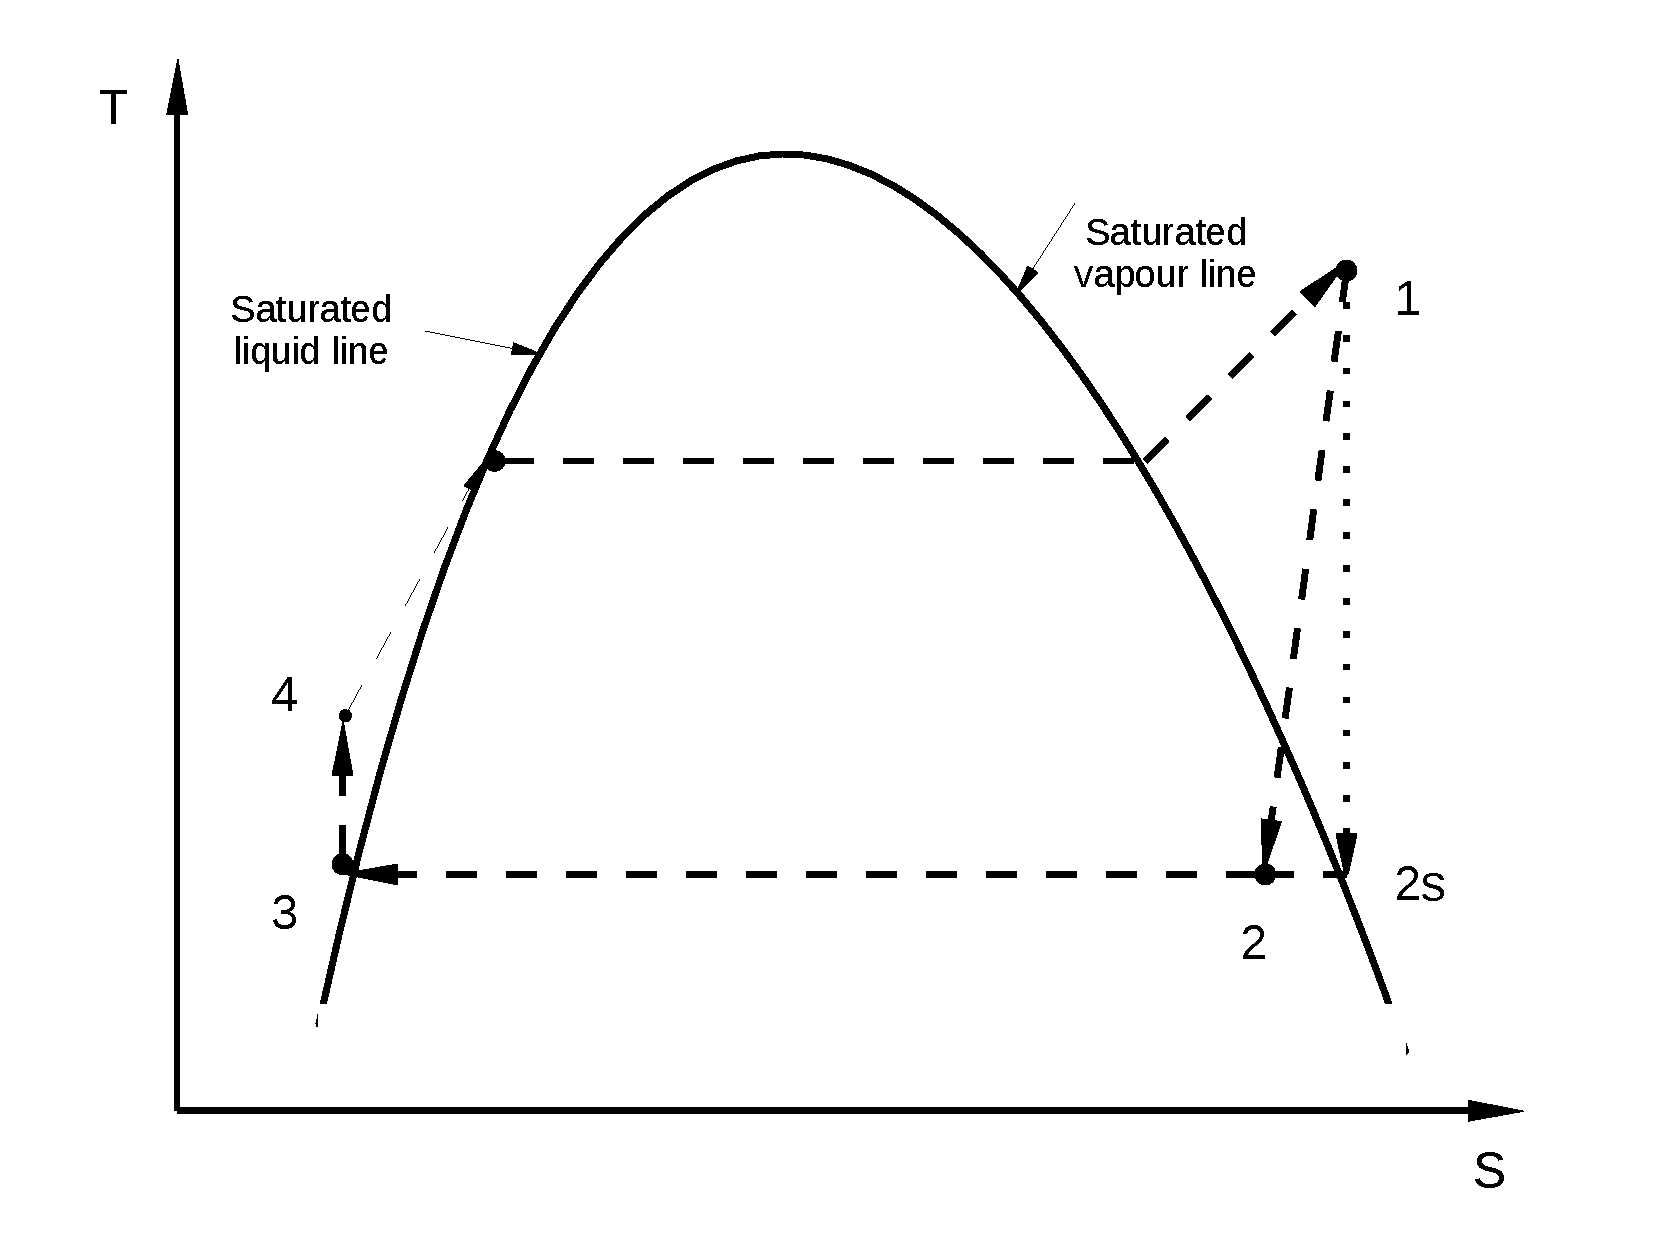
\includegraphics[width=8.cm,clip]{./Pics/TS_DIagramGeothermalBinary}
\end{center}%~\solmarks{3/3}
}
\end{enumerate} 

To solve this problem, you should assume that the saturated liquid streams are incompressible, and therefore $dH = VdP$ (where $H$, $V$ and $P$ are enthalpy, volume and pressure, respectively). Quality of the vapour is expressed as
\begin{displaymath}
x_{j} = \frc{\Psi_{j}-\Psi_{f}}{\Psi_{g}-\Psi_{f}}\;\;\;\text{with }\Psi=\left\{H,S\right\}
\end{displaymath}
where $S$ is the entropy. Efficiency of the turbine $\left(\eta_{\text{Turbine}}\right)$ and the heat exchanger $\left(\eta_{\text{HE}}\right)$ are given by,
\begin{displaymath}
\eta_{\text{Turbine}} =\frc{H_{2}-H_{1}}{H_{2s}-H_{1}} \;\;\;\text{ and }\;\;\; \eta_{\text{HE}} = \frc{\dot{Q}_{C3}}{\dot{Q_{gf}}}
\end{displaymath}
where $H_{2s}$ is the enthalpy of stream $2$ assuming ideal turbine performance (i.e., reversible expansion). $\dot{Q}_{C3}$ and $\dot{Q}_{gf}$ are the heat associated with the n-C$_{3}$ and brine streams, respectively, at the heat exchanger.

%
\end{question}

\clearpage
%%%
%%% Question 03
%%%
\begin{question}
\begin{enumerate}[(a)]
\item Develop expressions for the volume expansivity, $\beta=\frc{1}{V}\left(\frc{\partial V}{\partial T}\right)_{P}$, and isothermal compressibility, $\kappa=-\frc{1}{V}\left(\frc{\partial V}{\partial P}\right)_{T}$, for the following equations of state,
\begin{enumerate}[(i)]
\item ideal gas~\marks{4}
\solution{Ideal gas: $V=\frc{RT}{P}$,
\begin{displaymath}
\left(\frc{\partial V}{\partial T}\right)_{P} = \frc{R}{P} \;\;\; \left(\frc{\partial V}{\partial P}\right)_{T} = -\frc{RT}{P^{2}} 
\end{displaymath}~\solmarks{2/4}
Now deriving $\beta$ and $\kappa$,
\begin{displaymath}
{\bf \beta} = \frc{1}{V}\frc{R}{P} {\bf = \frc{1}{T}}\;\;\text{ and}\;\;\kappa = -\frc{1}{V}\left(-\frc{RT}{P^{2}}\right){\bf = \frc{1}{P}}
\end{displaymath}~\solmarks{2/4}
}
\item $V=\frc{RT}{P}+b$~\marks{4}
\solution{
The derivatives are,
\begin{displaymath}
\left(\frc{\partial V}{\partial T}\right)_{P} = \frc{R}{P} \;\;\; \left(\frc{\partial V}{\partial P}\right)_{T} = -\frc{RT}{P^{2}} 
\end{displaymath}~\solmarks{2/4}
Now deriving $\beta$ and $\kappa$,
\begin{displaymath} 
{\bf \beta} = \frc{1}{V}\frc{R}{P} =\frc{R}{V}\frc{V-b}{RT}= {\bf = \frc{1}{T}\frc{V-b}{V}} \;\;\text{ and }\;\; {\bf \kappa} = -\frc{1}{V}\left(-\frc{RT}{P^{2}}\right){\bf = \frc{1}{P}\left[\frc{V-b}{V}\right]}
\end{displaymath}~\solmarks{2/4}
}
\end{enumerate}

\item Calculate the compressibility factor ($Z$) of chloroform vapour at 450 K and 20 bar (molar volume of 1.35$\times$10$\left.^{-3}\text{ m}^{3}.\text{gmol}^{-1}\right)$ using the Soave-Redlich-Kwong equation of state. Properties of chloroform are: T$_{c}$ = 537 K, P$_{c}$ = 5328.68 kPa and $\omega$ =0.218 (accentric factor). In your iterative calculations, use $PV=ZRT$ as an initial guess of $Z$, and stop at the second iteration $\left(Z_{2}\right)$.~\marks{12}
\solution{ The generic form of $Z$ is,
\begin{displaymath}
Z = 1+ \beta - q\beta\frc{Z - \beta}{\left(Z+\epsilon\beta\right)\left(Z+\sigma\beta\right)}\;\;\text{ with} \;\; \beta = \Omega \frc{P_{r}}{T_{r}}\;\;\text{ and}\;\; q=\frc{\Psi\alpha}{\Omega T_{r}}
\end{displaymath}
For SRK with {\bf T$_{r}$=0.8380}, {\bf P$_{r}$=0.3754}, {\bf $\beta$=3.88$\times$10$^{-2}$} and {\bf $q$=6.7274}~\solmarks{2/12},
\begin{displaymath}
{\bf Z = 1 + \beta - q\beta\frc{Z-\beta}{Z^{2}+\beta Z}}
\end{displaymath}~\solmarks{2/12}
The equation is non-linear and to find the root we can apply Newton-Raphson method 
\begin{displaymath}
Z_{i} = Z_{i-1} - \frc{\mathcal{F}\left(Z_{i-1}\right)}{d\mathcal{F}/dZ \left(Z_{i-1}\right)}
\end{displaymath}
with,
\begin{eqnarray}
&& \mathcal{F}\left(Z\right) = Z - \left[ 1 + \beta - q\beta\frc{Z-\beta}{Z^{2}+\beta Z}\right] \nonumber \\
&& \frc{d\mathcal{F}}{dZ}\left(Z\right) = 1 + q\beta \frc{\beta^{2}+2\beta Z- Z^{2}}{\left(Z^{2}+\beta Z\right)^{2}} \nonumber
%\frc{q\beta\left(Z^{2}\beta +Z\right)-q\beta Z\left(2Z + \beta\right)}{\left(Z^{2}+\beta Z\right)^{2}} + \frc{q\beta^{2}\left(2Z+\beta\right)}{\left(Z^{2}+\beta Z\right)^{2}} \nonumber
\end{eqnarray} 
as initial guess, we can use the generic real gas EOS, $PV=Z_{0}RT \Longrightarrow$ {\bf $Z_{0}=0.7217$}~\solmarks{2/12}. Thus 
\begin{center}
{\bf $Z_{1}$ = 0.7184}~\solmarks{3/12} \\
{\bf $Z_{2}$ = 0.7160}~\solmarks{3/12} \\
$\cdots \cdots \cdots $ \\
\textcolor{red} {or (using calculator) }{\bf $Z_{22}$ = 0.7088}~\solmarks{\textcolor{red}{8/12}} \\

\end{center}
} 
\end{enumerate}

\end{question}

\clearpage

%%%
%%% Question 04
%%%
\begin{question}
 The excess molar volume of a solution of ethanol (1) and methyl-buthyl ether (2) at 298.15 K is given by the following expression:
\begin{displaymath}
\overline{V}^{\text{E}} =  x_{1}x_{2}\left[-1.026+0.22\left(x_{1}-x_{2}\right)\right]
\end{displaymath}
Given $\overline{V}_{1}=58.63$ cm$^{3}$.mol$^{-1}$ and $\overline{V}_{2}=118.46$ cm$^{3}$.mol$^{-1}$ $\left(\overline{V}_{i}\right.$ is the molar volume of component $i\left.\right)$.
\begin{enumerate}[(a)]
\item What is the volume of the solution when 750 cm$^{3}$ of pure ethanol is mixed with 1500 cm$^{3}$ of methyl-buthyl ether at 298.15 K?~\marks{14}
%
\solution{First, we need to calculate the number of moles $n= \frc{V}{\overline{V}}$ $\Longrightarrow$ {\bf n$_{1}$=12.79} and {\bf n$_{2}$=12.66} and the total number of moles $\left(n_{T}\right)$ is 25.455. The molar fraction can now be calculated as $x_{i}=n_{i}/n_{T}$ $\Longrightarrow$ {\bf x$_{1}$=0.5025} and {\bf x$_{2}$=0.4975}~\solmarks{4/14}. Substituting these values in,
\begin{displaymath}
{\bf \overline{V}^{\text{E}}} =  x_{1}x_{2}\left[-1.026+0.22\left(x_{1}-x_{2}\right)\right] {\bf = -0.2562 \frc{cm^{3}}{mol}}
\end{displaymath}~\solmarks{2/14}
The molar volume of the solution is given by
\begin{displaymath}
\overline{V}^{\text{E}} = \overline{V} - \sum\limits_{i=1}^{2}x_{i}\overline{V}_{i} \;\;\Longrightarrow \;\;\; {\bf \overline{V} = 88.1392\frc{cm^{3}}{mol}}
\end{displaymath}~\solmarks{2/14}
The total volume can then be calculated as 
\begin{displaymath}
{\bf V^{T}=\overline{V}.n_{T}=2243.5835\; cm^{3}}
\end{displaymath}~\solmarks{6/14} 
}
\item What would be the volume if the solution was ideal?~\marks{6}
\solution{The volume of the ideal solution is
\begin{displaymath}
{\bf V_{T}^{\text{ideal}}} = n_{T}\sum\limits_{i=1}^{2} x_{i}\overline{V}_{i} {\bf = 2250.1055\;cm^{3}}
\end{displaymath}~\solmarks{6/6}
}
\end{enumerate}
%
\end{question}

\clearpage

%%%
%%% Question 05
%%%

\begin{question}
A mixture of 2 kg of H$_{2}$ and 4 kg of N$_{2}$ was compressed in a piston-cylinder in a polytropic process with $n=1.2$. During the compression, the temperature increased from 22 to 150$^{\circ}$C. Determine the heat transfer (in {\it kJ}) and the entropy change (in $kJ/K$) of the process. The entropy change is expressed as,
\begin{displaymath}
\Delta S = m_{T}\left[\overline{C}_{v}\ln\frc{T_{2}}{T_{1}}+\frc{R}{\overline{MW}}\ln\frc{V_{2}}{V_{1}}\right] 
\end{displaymath}
where $m_{T}$ is the total mass of the gaseous mixture, $\overline{MW}$ and $\overline{C}_{v}$ are the averaged molar mass and heat capacity at constant volume of the mixture. For this range of temperature, you should assume constant heat capacity at constant volume $\left(C_{v}\right)$ of 0.745 and 10.32 kJ.(kg.K)$^{-1}$, for N$_{2}$ and H$_{2}$, respectively. Molar mass of H$_{2}$: 2.016 g.mol$^{-1}$, N$_{2}$: 28.01 g.mol$^{-1}$.~\marks{20}
\solution{For H$_{2}$ (1) and N$_{2}$ (2), n$_{1}$ = 0.9921,  n$_{2}$=0.1428 and n$_{T}$ = 1.1349 (also m$_{T}$ = 6kg) $\Longrightarrow$ ${\bf y_{1}=0.8742}$ and ${\bf y_{2}=0.1258}$~\solmarks{2/20}. Now we can calculate the averaged molecular weight $\overline{MW}$,
\begin{displaymath}
{\bf \overline{MW}} = \sum\limits_{i=1}^{2} y_{i} MW_{i} {\bf = 5.2860\frc{kg}{kgmol}} 
\end{displaymath}~\solmarks{2/20}
and
\begin{displaymath}
\overline{C}_{v}=  \sum\limits_{i=1}^{2} y_{i} C_{v,i} = 9.1155 \frc{kJ}{kg.K}
\end{displaymath}
From the first law, $dU = dQ - dW$, for the polytropic compression $\left(PV^{n}=C\right)$ we need work to be executed,
\begin{eqnarray}
dW = PdV \Longrightarrow {\bf W} &=& \int\limits_{1}^{2} P dV = \int\limits_{1}^{2} \frc{C}{V^{n}}dV = \left.\frc{CV^{1-n}}{1-n}\right|_{1}^{2}=\left.\frc{PV}{1-n}\right|_{1}^{2}=\left.\frc{n_{T}RT}{1-n}\right|_{1}^{2} \nonumber \\
                           &=& \frc{m_{T}}{\overline{MW}}\frc{R\left(T_{2}-T_{1}\right)}{1-n} {\bf = -6038.98 kJ} \nonumber
\end{eqnarray}~\solmarks{4/20}
The variation in internal energy can be calculated as,
\begin{displaymath}
{\bf \Delta U} = \sum\limits_{i=1}^{2} m_{1}C_{v,i} \Delta T {\bf = 3023.36 kJ}
\end{displaymath}~\solmarks{4/20}
Thus, the heat is 
\begin{displaymath}
{\bf Q} =\Delta U + W {\bf = -3016.62 kJ}
\end{displaymath}~\solmarks{4/20}
Now to calculate the variation in entropy,
\begin{eqnarray}
{\bf \Delta S} &=& m_{T}\left[\overline{C}_{v}\ln\frc{T_{2}}{T_{1}}+\frc{R}{\overline{MW}}\ln\frc{V_{2}}{V_{1}}\right] = m_{T}\left[\overline{C}_{v}\ln\frc{T_{2}}{T_{1}}+\frc{R}{\overline{MW}}\ln\left(\frc{T_{1}}{T_{2}}\right)^{\frc{1}{n-1}}\right]\nonumber  \nonumber \\
               &=& m_{T}\left[\overline{C}_{v}-\frc{\frc{R}{\overline{MW}}}{n-1}\right]\ln\frc{T_{2}}{T_{1}} {\bf = 2.7042 \frc{kJ}{K}}\nonumber 
\end{eqnarray}~\solmarks{4/20}
}


\end{question}
%\begin{comment}
\clearpage
\begin{itemize}
%%%
\item Generic cubic equation of state:
\begin{eqnarray}
&& Z= 1 + \beta - q\beta \frc{Z - \beta} {\left(Z+\varepsilon\beta\right)\left(Z+\sigma\beta\right)}  \;\;\text{(vapour and vapour-like roots)}\nonumber\\
&& Z= 1 + \beta + \left(Z + \epsilon\beta\right)\left(Z+\sigma\beta\right)\left(\frc{1+\beta-Z}{q\beta}\right)  \;\;\text{(liquid and liquid-like roots)}\nonumber\\
&& \text{with }\; \beta=\Omega\frc{P_{r}}{T_{r}} \;\;\text{ and } \;\; q=\frc{\Psi\alpha\left(T_{r}\right)}{\Omega T_{r}}  \nonumber \\
&&\alpha_{\text{SRK}} = \left[ 1 + \left( 0.480 + 1.574 \omega - 0.176\omega^{2}\right)\left(1-\sqrt{T_{r}}\right)\right]^{2}  \nonumber \\
&&\alpha_{\text{PR}} = \left[ 1 + \left( 0.37464 + 1.54226 \omega - 0.26992\omega^{2}\right)\left(1-\sqrt{T_{r}}\right)\right]^{2} \nonumber
\end{eqnarray} 
    \begin{center}
       \begin{tabular}{| l | c c c c c| }
       \hline
          {\bf EOS}  & {\bf $\alpha$} & {\bf $\sigma$}  & {\bf $\varepsilon$} & {\bf $\Omega$} & {\bf $\Psi$ } \\
       \hline
            vdW      & 1              & 0               & 0                  & 1/8            & 27/64          \\
            RK       & T$_{r}^{-1/2}$  & 1                & 0                  & 0.08664       & 0.42748        \\
           SRK       &$\alpha_{\text{SRK}}$& 1            & 0                   & 0.08664       & 0.42748        \\
            PR       &$\alpha_{\text{PR}}$& 1+$\sqrt{2}$   & 1-$\sqrt{2}$        & 0.07780        & 0.45724  \\
       \hline
       \end{tabular}
    \end{center}

%%%
\item Newton-Raphson (root-finder) method: $X_{i} = X_{i-1} - \frc{\mathcal{F}\left(X_{i-1}\right)}{d\mathcal{F}/dX\left(X_{i-1}\right)}$

%%%
\item Fundamental thermodynamic equations:\\
\begin{tabular}{c c c c}
$dU = dQ + dW$;  & $dH = dU + d(PV)$; & $dA = dU -d(TS)$; & $dG=dH-d(TS)$ \\
$dU = TdS - PdV$;& $dH = TdS + VdP$;  & $dA = -SdT - PdV$;& $dG = -SdT + VdP$ \\ 
\end{tabular}\\
\begin{tabular} {c c}
$dH = C_{p}dT + \left[ V - T\left(\frc{\partial V}{\partial T}\right)_{P}\right]dP$; &  $dS=C_{p}\frc{dT}{T} - \left(\frc{\partial V}{\partial T}\right)_{P}dP$ \\
$dU = C_{v}dT + \left[T\left(\frc{\partial P}{\partial T}\right)_{V} - P\right]dV$;  & $dS = C_{v}\frc{dT}{T} - \left(\frc{\partial P}{\partial T}\right)_{V}dV$
\end{tabular}

%%% 
\item Polytropic Relations:\\
\begin{displaymath} 
\frc{T_{2}}{T_{1}} =\left(\frc{P_{2}}{P_{1}}\right)^{\frac{\gamma-1}{\gamma}} = \left(\frc{V_{1}}{V_{2}}\right)^{\gamma-1}\;\; ; 
TV^{\gamma-1} =\text{ const};\; TP^{\frac{1-\gamma}{\gamma}}=\text{ const};\; PV^{\gamma}=\text{ const} 
\end{displaymath}

%%%
\item Raoult's Law:\\
\begin{displaymath}
y_{i}P = x_{i}P_{i}^{\text{sat}}\;\;\;\text{ and } \;\;\; y_{i}P = x_{i}\gamma_{i}P_{i}^{\text{sat}}\;\;\;\text{ with } i=1,2,\cdots N
\end{displaymath}

%%%
\item Henry's Law:\\
\begin{displaymath}
x_{i}\mathcal{H}_{i} = y_{i}P\;\;\;\text{ with } i=1,2,\cdots N
\end{displaymath}

%%%
\item Antoine Equation:\\
\begin{displaymath}
\log_{10} P^{\star} = A-\frc{B}{T+C}\;\;\;\text{ with P}^{\star}\text{ in mm-Hg and T in }^{\circ}\text{C}
\end{displaymath}

%%%
\item Solutions:\\
\begin{displaymath}
M^{\text{E}} = M - \sum\limits_{i=1}^{N} x_{i}M_{i}; \; \overline{M}_{1}=M+x_{2}\frc{d M}{dx_{1}};\; \overline{M}_{2} = M - x_{1}\frc{d M}{dx_{1}}
\end{displaymath}

\end{itemize}

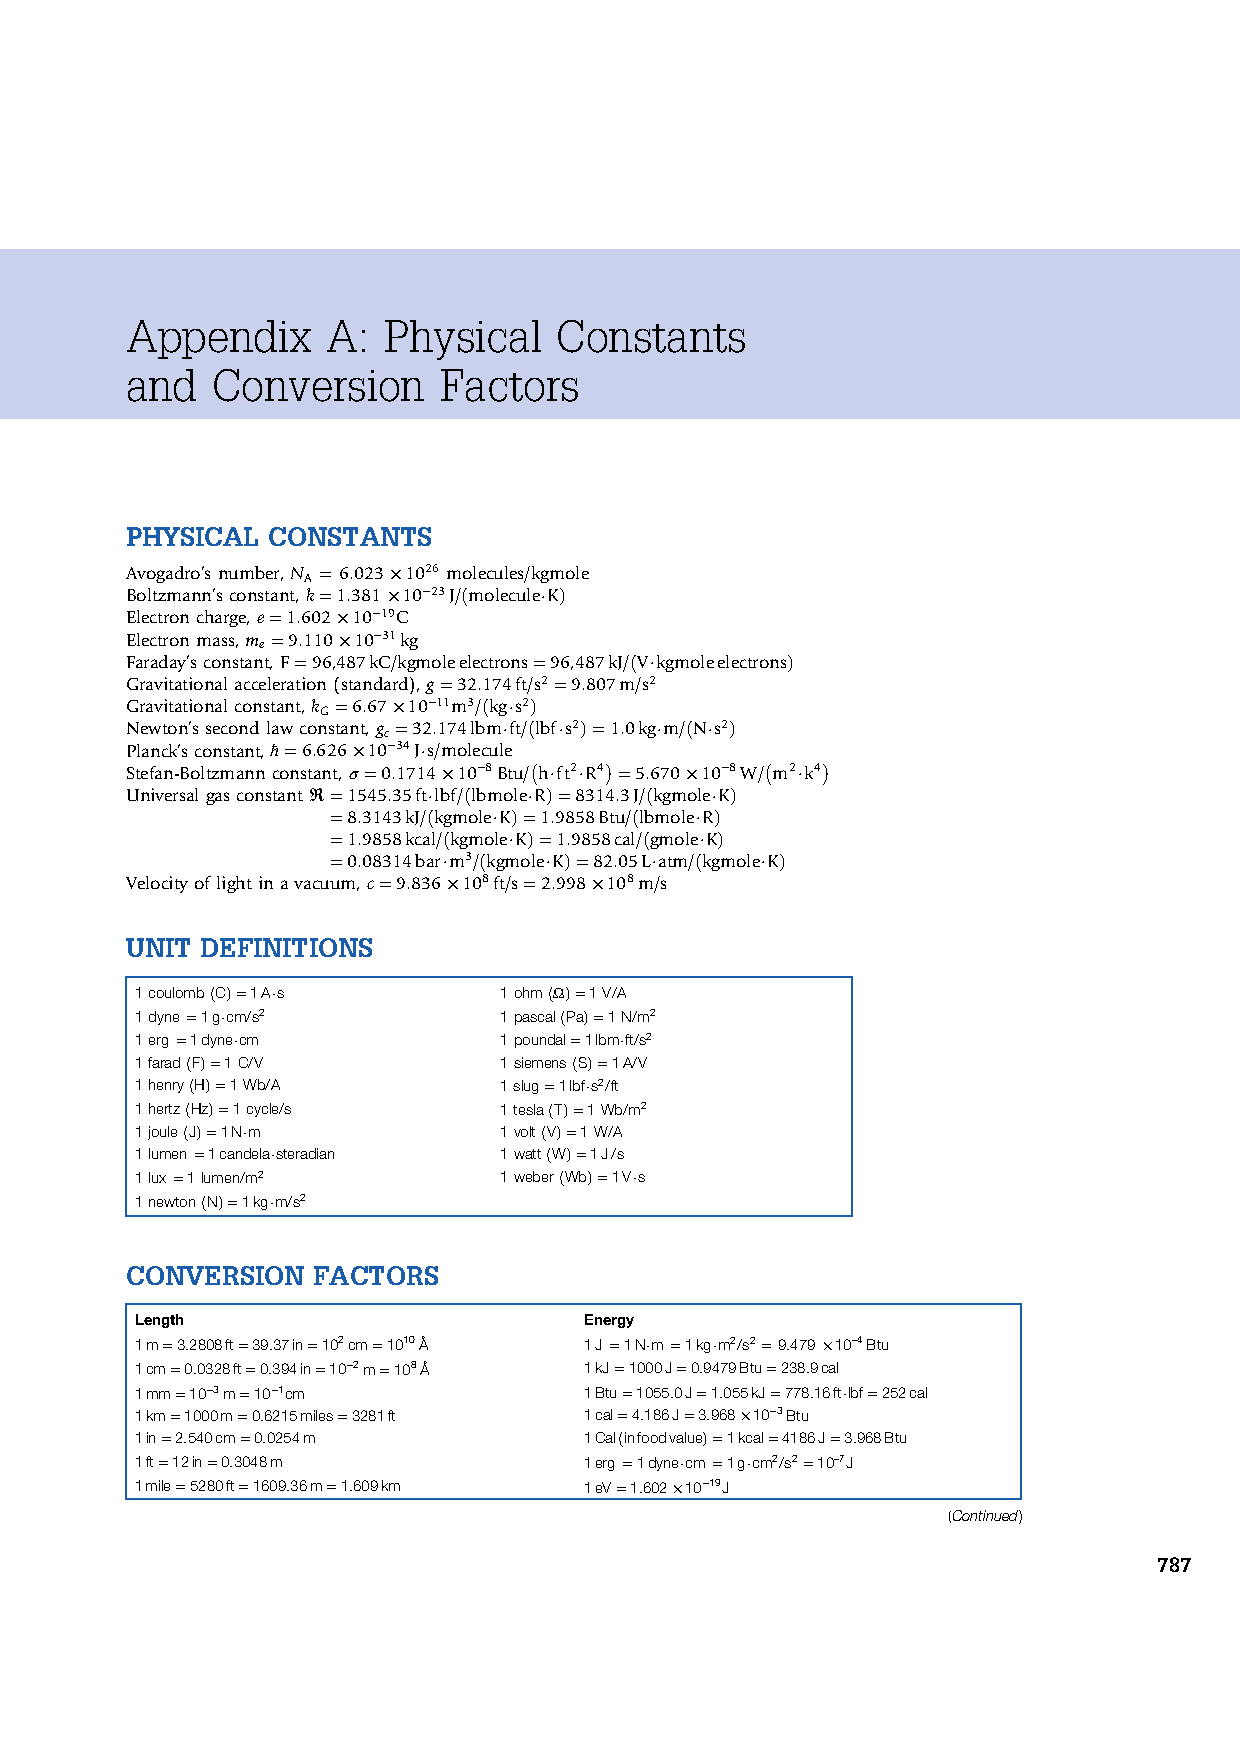
\includepdf[pages={1-6}]{./Pics/nC3_UnitConv}
%\end{comment}
\clearpage
\end{document}
